%
% File emnlp2016.tex
%

\documentclass[11pt,letterpaper]{article}

\usepackage{emnlp2016}
\usepackage{times}
\usepackage{latexsym}

% reference appendix
\usepackage{xr}
\externaldocument{supplemental}

% \RequirePackage[l2tabu, orthodox]{nag}
% \documentclass{article}

% % FONTS
\usepackage[T1]{fontenc}

% Replace default Latin Modern typewriter with its proportional counterpart
% http://www.tug.dk/FontCatalogue/lmoderntypewriterprop/
\renewcommand*\ttdefault{lmvtt}

%\usepackage[bitstream-charter]{mathdesign} % not needed for mtpro
\usepackage{amsmath}
\usepackage[subscriptcorrection,
            amssymbols,
            mtpbb,
            mtpcal,
            nofontinfo  % suppresses all warnings
           ]{mtpro2} %TODO: put htis back in and take out mathdesign
\usepackage{scalefnt,letltxmacro}
\LetLtxMacro{\oldtextsc}{\textsc}
\renewcommand{\textsc}[1]{\oldtextsc{\scalefont{1.10}#1}}
\usepackage[scaled=0.92]{PTSans}


% % COLOR
\usepackage[usenames,dvipsnames]{xcolor}
\definecolor{Green}{HTML}{156946}

% % SPACING and TEXT
\usepackage[final,expansion=alltext]{microtype}
\usepackage[english]{babel}
\usepackage{afterpage}
\usepackage{framed}


% define a paragraph header function
\DeclareRobustCommand{\parhead}[1]{\textbf{#1}~}

% % EDITING
% paragraph helper
\DeclareRobustCommand{\PP}{\textcolor{Plum}{\P} }

% % COUNTERS
\usepackage{enumitem}
\renewcommand{\labelenumi}{\color{black!67}{\arabic{enumi}.}}
\renewcommand{\labelenumii}{{\color{black!67}(\alph{enumii})}}
\renewcommand{\labelitemi}{{\color{black!67}\tiny$\blacksquare$}}
\renewcommand{\labelitemii}{{\color{black!67}\textbullet}}
\renewcommand{\labelitemiii}{{\color{black!67}\scriptsize$\blacktriangleright$}}

% FIGURES
\usepackage{graphicx}

% TABLES
\usepackage{booktabs}

% ALGORITHMS
\usepackage[algoruled]{algorithm2e}
\usepackage{listings}
\usepackage{fancyvrb}
\fvset{fontsize=\normalsize}

% % HYPERREF
\usepackage[colorlinks,linktoc=all]{hyperref} %TODO: rm draft
\usepackage[all]{hypcap}
\hypersetup{citecolor=Green}
\hypersetup{linkcolor=Green}
\hypersetup{urlcolor=Green}

% % CLEVEREF must come after HYPERREF
\usepackage[nameinlink]{cleveref}

% BIBLIOGRPHY: get rid of reference labels
\makeatletter
	\renewcommand\@biblabel[1]{}
\makeatother

% ACRONYMS
\usepackage[acronym,smallcaps,nowarn]{glossaries}
% \makeglossaries

% % COLOR DEFINITIONS
\newcommand{\green}[1]{\textcolor{Green}{#1}}


% LISTINGS DEFINTIONS
\lstdefinestyle{mystyle}{
    commentstyle=\color{Green},
    keywordstyle=\color{Green},
    numberstyle=\tiny\color{black!60},
    stringstyle=\color{Green},
    basicstyle=\ttfamily,
    breakatwhitespace=false,
    breaklines=true,
    captionpos=b,
    keepspaces=true,
    numbers=left,
    numbersep=5pt,
    showspaces=false,
    showstringspaces=false,
    showtabs=false,
    tabsize=2
}
\lstset{style=mystyle}

% ALGORITHMS
\usepackage[algoruled]{algorithm2e}

% FRAMES
\usepackage[linewidth=1pt]{mdframed}
\DeclareRobustCommand{\mb}[1]{\ensuremath{\boldsymbol{\mathbf{#1}}}}

\DeclareMathOperator*{\argmax}{arg\,max}
\DeclareMathOperator*{\argmin}{arg\,min}

\DeclareRobustCommand{\KL}[2]{\ensuremath{\textrm{KL}\left(#1\;\|\;#2\right)}}

\newcommand{\mbx}{\mathbold{x}}
\newcommand{\mbX}{\mbf{X}}

\newcommand{\mbz}{\mathbold{z}}

\newcommand{\mbI}{\mbf{I}}

\newcommand{\mbZ}{\mbf{Z}}
\newcommand{\mbL}{\mbf{L}}

\newcommand{\mbtheta}{\mathbold{\theta}}
\newcommand{\mbTheta}{\mathbold{\Theta}}
\newcommand{\mbomega}{\mathbold{\omega}}
\newcommand{\mbOmega}{\mathbold{\Omega}}
\newcommand{\mbsigma}{\mathbold{\sigma}}
\newcommand{\mbSigma}{\mathbold{\Sigma}}

\newcommand{\mblambda}{\mathbold{\lambda}}
\newcommand{\mbgamma}{\mathbold{\gamma}}
\newcommand{\mbzeta}{\mathbold{\zeta}}
\newcommand{\mbeta}{\mathbold{\eta}}
\newcommand{\mbbeta}{\mathbold{\beta}}
\newcommand{\mbphi}{\mathbold{\phi}}
\newcommand{\mbmu}{\mathbold{\mu}}
\newcommand{\mbrho}{\mathbold{\rho}}

\newcommand\dif{\mathop{}\!\mathrm{d}}
\newcommand{\diag}{\textrm{diag}}
\newcommand{\supp}{\textrm{supp}}

\newcommand{\E}{\mathbb{E}}
\newcommand{\Var}{\mathbb{V}\textrm{ar}}

\newcommand{\bbN}{\mathbb{N}}
\newcommand{\bbZ}{\mathbb{Z}}
\newcommand{\bbR}{\mathbb{R}}
\newcommand{\bbS}{\mathbb{S}}

\newcommand{\cL}{\mathcal{L}}

\newcommand{\cN}{\mathcal{N}}
\newcommand{\Gam}{\textrm{Gam}}
\newcommand{\InvGam}{\textrm{InvGam}}

\newcommand{\g}{~\vert~}
\newacronym{KL}{kl}{Kullback-Leibler}
\newacronym{ELBO}{elbo}{\emph{evidence lower bound}}
\newacronym{POPELBO}{pop-elbo}{\emph{population evidence lower bound}}

\newacronym{SVI}{svi}{stochastic variational inference}
\newacronym{BUMPVI}{bump-vi}{bumping variational inference}

\newacronym{GMM}{gmm}{Gaussian mixture model}
\newacronym{LDA}{lda}{latent Dirichlet allocation}

\newacronym{SUTVA}{sutva}{stable unit treatment value assumption}


% Uncomment this line for the final submission:
\emnlpfinalcopy

%  Enter the EMNLP Paper ID here:
\def\emnlppaperid{***} % TODO


\title{Detecting and Characterizing Events}

\author{
Allison J.~B. Chaney\\
    Princeton University\\
	\href{mailto:achaney@cs.princeton.edu}{\nolinkurl{achaney@cs.princeton.edu}}
\And
Hanna Wallach\\
    Microsoft Research\\
    \href{mailto:wallach@microsoft.com}{\nolinkurl{wallach@microsoft.com}}
\AND
Matthew Connelly\\
    Columbia University\\
    \href{mailto:mjc96@columbia.edu}{\nolinkurl{mjc96@columbia.edu}}
\And
David M. Blei\\
    Columbia University\\
    \href{mailto:david.blei@columbia.edu}{\nolinkurl{david.blei@columbia.edu}}
}

\date{}

\begin{document}

\maketitle

\begin{abstract}
%!TEX root = emnlp2016.tex

Significant events are characterized by interactions between entities (e.g., countries, organizations, individuals) that deviate from typical interaction patterns.  Investigators, such as historians, commonly read large quantities of text to construct an accurate picture of who, what, when, and where and event happened.  In this work, we present the Capsule model for analyzing documents to identify and characterize events of potential significance.
Specifically, we develop a model based on topic modeling to distinguish between topics that describe ``business-as-usual'' and topics that deviate from these patterns.
To demonstrate this model, we analyze a corpus of over 2 million US State Department cables from the 1970s; we provide open-source implementations of an inference algorithm for the Capsule model and a pipeline to explore its results.
\end{abstract}


\section{Introduction}
\label{sec:intro}
%!TEX root = emnlp2016.tex

% TODO | fill in the XXX below

% TODO | fill in with real cables

Foreign embassies of the United States government communicate with
each other and with the U.S. State Department through cabled message.
The National Archive collects these documents in a running corpus,
which traces the (unclassified) diplomatic history of the United
States. Between 1973 and 1978, for example, it has collected about two
million cables.

Typically, a cable from this collection describes diplomatic ``business as usual,'' such as arrangements for visiting officials, recovery of lost or stolen passports, or obtaining lists of names for meetings and conferences. For example,
the embassies sent 8,635 cables during the week of April 21, 1975. Here is one,
selected at random,
\begin{shaded*} \tt{Hoffman, UNESCO Secretariat, requested info from
PermDel concerning an official invitation from the USG
RE subject meeting scheduled 10-13 JUNE 1975, Madison,
Wisconsin.  Would appreciate info RE status of action to 
be taken in order to inform Secretariat.  Hoffman communicating 
with Dr.~John P.~Klus RE list of persons to be invited.}
\end{shaded*}

But hidden in the corpus are also cables about important diplomatic
events, the cables and events that are of primary interest to
historians. During that same week the United States was in the last
moments of the Vietnam war and, on April 30, 1975, lost its hold on Saigon. This resulted in the end of the Vietnam War and a max exodus of refugees from the country.  One
of the cables around this event is
\begin{shaded*}
  \tt{GOA program to move Vietnamese Refugees to Australia
  is making little progress and probably will not cover more than
  100-200 persons.  Press comment on smallness of program has
  recognized difficulty of getting Vietnamese out of Saigon, but
  ``Canberra Times'' Apr 25 sharply critical of government's
  performance.  [...]
  %Opposition continues to attack smallness of program,
  %but seems concerned, as does government, with scoring
  %point of domestic political importance.  With Parliament in
  %recess for next three weeks and Prime Minister on trip, issue
  %may attract less attention.
  Labor government clearly hopes whole
  matter will somehow disappear.}
\end{shaded*}

% cheating by putting this here...
\begin{figure*}[ht]
\centering
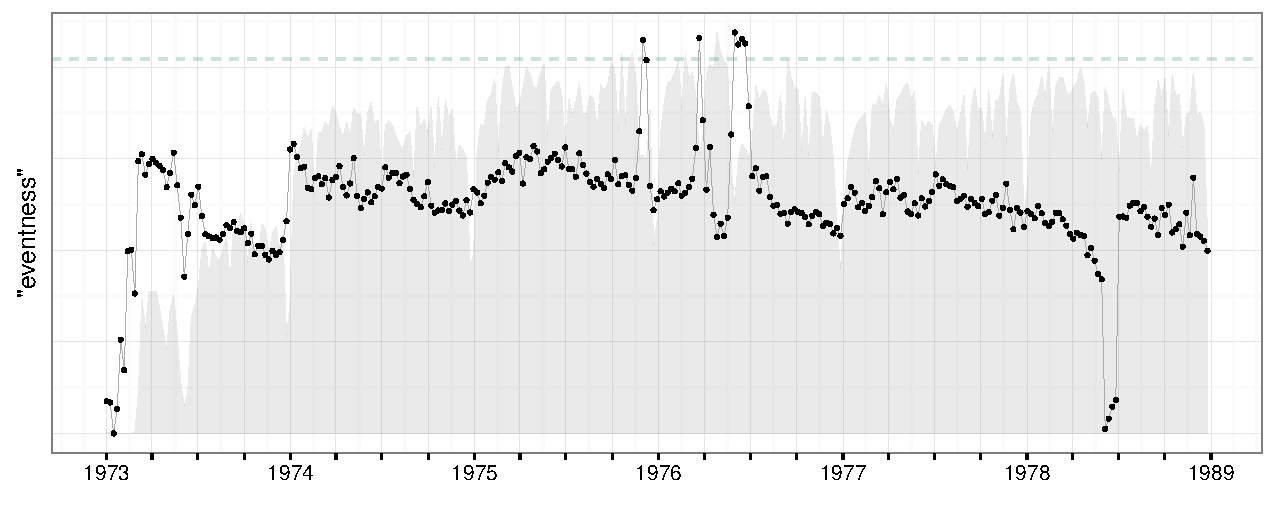
\includegraphics[width=\linewidth]{fig/cables_events.pdf}
\caption{Measure of time interval impact on cable content: $\psi_t \frac{1}{\vert D_t \vert}\sum_{d\in D_t} \epsilon_{d,t}$, where $D_t$ is the set of all cables sent in interval $t$.  The grey background indicates the number of cables sent over time.}
\label{fig:cables_events}
\end{figure*}

Our goal in this paper is to develop a method to help historians and
political scientists wade through their collections, such as the 1970s
cables, to find potentially important events, such as the fall of
Saigon, and the primary sources around them. We develop
\textit{Capsule}, a probabilistic model for detecting and
characterizing important events in large collections of historical
communication.

\Cref{fig:cables_events} illustrates Capsule's analysis of the two
million cables from the National Archives. The $y$-axis is
``eventness'', a loose measure how strongly a week's cables deviate
from the usual diplomatic chatter to discuss a matter that is common
to many embassies. (This is described in detail in \Cref{}.)

The figure shows that Capsule detects many of the important moments
during this five-year span, including Indonesia's invasion of East
Timor (XXX), the Air France hijacking and Israeli rescue operation
(XXX), and the fall of Saigon (XXX). It also identifies other moments,
such as the U.S. sharing lunar rocks with other countries (XXX) and
the death of Mao Tse-tung (XXX). Broadly speaking, Capsule gives a
picture of the diplomatic history of these five years; it identifies
and characterizes moments and source material that might be of
interest to a historian.

The intuition behind Capsule is this. Embassies write cables
throughout the year, usually describing typical business such as the
visiting of a government official. Sometimes, however, there is an
important event---e.g., the fall of Saigon. When an event occurs, it
pulls embassies away from their typical business to write cables that
discuss what happened and its consequences. Thus Capsule effectively
defines an ``event'' to be a moment in history when embassies deviate
from what each usually discusses, and when each embassy deviates in
the same way.

Capsule embeds this intuition into a Bayesian model. It uses hidden
variables to encode what ``typical business'' means for each embassy,
how to characterize the events of each week, and which cables discuss
those events. Given a corpus, the corresponding posterior distribution
provides a filter on the cables that isolates important moments in the
diplomatic history. \Cref{fig:cables_events} illustrates this
posterior.

% TODO | mention that this can be used with other types of corpora

% TODO | summary of the paper's sections

\parhead{Related work.} We first review previous work on automatic
event detection and other related concepts.

% While Capsule uses text documents and associated metadata as input, event detection is often performed with univariate input data.  In this context, bursts that deviate from typical behavior (e.g., noisy constant or a repeating pattern) can define an event \cite{kleinberg2003bursty,ihler2007learning}; Poisson Processes~\cite{Kingman:1993} are often used to model events under this definition.  Alternatively, events can be construed as ``change points'' to mark when typical observations shift semi-permanently from one value to another~\cite{guralnik1999event}.
In both univariate and multivariate settings, the goal is often the same: analysts want to predict whether or not a rare events will occur~\cite{weiss1998learning,das2008anomaly}.  Capsule, in contrast, is designed to help analysts explore and understand the original data: our goal is interpretability, not prediction.

% Text is often used in event detection, as it is an abundant source of data.  
% In some applications, documents themselves are considered to be observed events~\cite{mccallum1998comparison,peng2007event}, or events are predetermined and tracked through the documents~\cite{yang2000improving,VanDam:2012}.  We are interested in detecting \emph{unobserved} events which can be characterized by patterns in the data.
%\newpage % note:when using hyperref, references can be split between pages!
A common goal is to identify clusters of documents; these approaches are used on news articles~\cite{zhao2012novel,zhao2007temporal,zhang2002novelty,li2005probabilistic,wang2007mining,allan1998line} and social media posts~\cite{VanDam:2012,lau2012line,jackoway2011identification,sakaki2010earthquake,reuter2012event,becker2010learning,sayyadi2009event}.  
In the case of news articles, the task is to create new clusters as novel news stories appear---this does not help disentangle typical content from rare events of interest.
Social media approaches identify rare events, but the methods are designed for short, noisy documents; they are not appropriate for larger documents that contain information about a variety of subjects.

Many existing methods use document terms as features, frequently weighted by tf-idf value~\cite{fung2005parameter,kumaran2004text,brants2003system,das2011dynamic,zhao2007temporal,zhao2012novel}; here, events are bursts in groups of terms. % Because language is high dimensional, using terms as features limits scalability.

Topic models~\cite{Blei:2012} reduce the dimensionality of text data; they have been used to help detect events mentioned in social media posts~\cite{lau2012line,dou2012leadline} and posts relevant to monitored events~\cite{VanDam:2012}.
We rely on topic models to characterize both typical content and events, but grouped observations can also be summarized directly~\cite{peng2007event,chakrabarti2011event,gao2012joint}.

In addition to text data over time, author~\cite{zhao2007temporal}, news outlet~\cite{wang2007mining}, and spatial information~\cite{Neill:2005,mathioudakis2010identifying,liu2011using} can be used to augment event detection.  Capsule uses author information in order to characterize typical concerns of authors.

Detecting and characterizing relationships~\cite{schein2015bayesian,linderman2014discovering,das2011dynamic} is related to event detection.  When a message recipient is known, Capsule's author input can be replaced with a sender-receiver pair, but the model could be further tailored for interactions within networks.

% Once events have been identified and characterized, visualization translates a model's output into sometime intepretable for non experts.  LeadLine~\cite{dou2012leadline} is an excellent example of a visualization of event detection.  We build on topic model visualization concepts~\cite{chaney2012visualizing} to provide tailored visualization code for Capsule.

% ===== old introduction

% Events are difficult to define; historians and political scientists read large quantities of text to construct an accurate picture of a single historical event.  Events are interesting by definition: they are the hidden causes of anomalous observations.  But they are also inherently abstract---we can observe that changes occur, but we cannot directly observe whether or not an event occurs.

% Consider embassies sending diplomatic messages, such as shown in Figure~\ref{fig:cartoon}.  The Bangkok embassy, Hong Kong Embassy, and the State Department all have \emph{typical concerns} about which they usually send messages.  At date $d$, however, the message content changes for all three entities---again, we only observe the changes in message content, and do not observe the event directly.  Our first goal is to determine \emph{when} events happen, or identify these rare but pervasive deviations from the typical concerns.

% Our second goal is to characterize \emph{what} occurs.  We rely on topic modeling~\cite{Blei:2012} to summarize content and to characterize events.

% We develop a Bayesian model that discovers the typical concerns of authors, identifies when events occur, and characterizes these events; we call this the \emph{Capsule} model, as it encapsulates events.

% %Our final goal is to visualize the results of the Capsule model to make them accessible.   We provide source code for both Capsule and its associated visualization.

% We first review previous research related to event detect, summarization, and visualization.  In Section~\ref{sec:model}, we describe the Capsule model and how to infer the latent parameters (the appendix provides further inference details).  Section~\ref{sec:eval} provides an exploration of results on simulated and a real-world data set, and we conclude with a discussion in Section~\ref{sec:discussion}.

% % Contributions
% % \begin{itemize}
% % \item we define the concept of events via our model
% % \item inference + code for this model
% % \item (hopefully) evidence that our model outperfoms baselines in terms of event detection
% % \item exploration of cables (+ other)
% % \item visualization / exploration pipeline for investigating a generic corpus fit
% % \end{itemize}


% % \PP outliers vs events \cite{Neill:2009} (univariate -> multivariate); this whoudlbe in reated work?
% % How is event detection different from:
% % 1. SupervisedLearning:
% % • Abnormal events are extremely rare, normal events are
% % plentiful
% % 2. Clustering:
% % • Clustering = partitioning data into groups
% % • Not the same as finding statistically anomalous groups
% % 3. OutlierDetection:
% % • Events of interest are usually not individual outliers
% % • The event typically affects a subgroup of the data rather than a single data point

%%% Local Variables:
%%% mode: latex
%%% TeX-master: "emnlp2016"
%%% End:


\section{The Capsule Model}
\label{sec:model}
%!TEX root = emnlp2016.tex

In this section, we present the Capsule model for detecting and
characterizing significant diplomatic events. We first provide the
intuition behind Capsule, and then formally specify the model. We also
explain how to use Capsule to explore a corpus and how to learn the
posterior distribution of the latent variables.

\begin{figure}
\centering
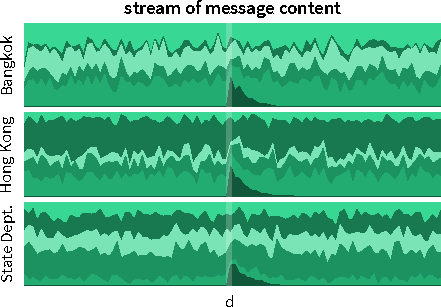
\includegraphics[width=\linewidth]{fig/cartoon.pdf}
\caption{Cartoon intuition. The $y$-axis represents the stacked
  proportions of cables about various topics, while the $x$-axis
  represents time. The Bangkok embassy, Honk Kong embassy, and
  U.S. State Department all have typical diplomatic business, about
  which they usually send cables. When an event occurs during time
  interval $t$, the cables alter to cover the event before returning
  to ``business as usual.'' Capsule discovers the embassies' typical
  concerns, as well as the timing and content of events.}
\label{fig:cartoon}
\end{figure}

Consider an entity like the Bangkok embassy, as illustrated in
\cref{fig:cartoon}. We can imagine that this entity sends a stream of
diplomatic cables over time---some to the U.S. State Department,
others to other American embassies, such as the one in Hong
Kong. Embassies usually write cables that describe typical diplomatic
business. For example, the Bangkok embassy might write about topics
regarding southeast Asia more generally. We can think of a topic as
being a probability distribution over vocabulary terms.

Now imagine that an event, such as the capture of Saigon during the
Vietnam war, occurs during a particular time interval $t$. We cannot
directly observe the occurrence of this event, but we can observe the
stream of cables and the event's impact on it. When the event occurs,
multiple entities deviate from their usual topics of discussion
simultaneously, before returning to their usual behavior, as depicted
in \cref{fig:cartoon}. For example, the day after the capture of
Saigon, the majority of the diplomatic cables written by the Bangkok
embassy and several other entities were about Vietnam war refugees. If
we think of the event as another probability distribution over
vocabulary terms, then each entity's stream of cables reflects its
typical concerns, as well as any significant events.


% \parhead{Background: Topic Models.} Capsule builds on topic models.  Topic models are algorithms for discovering the main themes in a large collection of documents; each document can then be summarized in terms of the global themes.  More formally, a topic $k$ is a probability distribution over the set of vocabulary words.  Each document $d$ is represented as a distribution over topics $\theta_d$.  Thus we can imagine that when we generate a document, we first pick which topics are relevant (and in what proportions).  Under the LDA topic model~\cite{Blei:2003}, we know the number of words in each document.  Then, for each word, we select a single topic from this distribution over topics, and finally select a vocabulary term from the corresponding topic's distribution over the vocabulary.  Alternatively, we can cast topic modeling as factorization, such as in Poisson factorization~\cite{Gopalan:2014b}, and draw a word count for each term in the vocabulary.

% Topic models are often applied to provide a structure for an
% otherwise unstructured collection of documents.  Documents, however,
% are often accompanied by metadata, such as the date written or
% author attribution; this information is not exploited by traditional
% topic models.  The Capsule model uses both author and date
% information to identify and characterize events that influence the
% content of the collection.

\subsection{Model Specification}
\label{sec:model_spec}

We now define the Capsule model. Our data come from \emph{entities}
(e.g., embassies) who send \emph{messages} (e.g., diplomatic cables)
over \emph{time}; specifically, we observe the number of times
$n_{dv}$ that each vocabulary term $v$ occurs in each message
$d$. Each message is associated with an author entity $a_d$ and a time
interval $t_d$ within which that message was sent.

We model each message with a bank of Poisson distributions---one for
each vocabulary term:
\begin{align}
  n_{dv} \sim \textrm{Poisson}\left(\lambda_{dv}\right).
\end{align}
The rate $\lambda_{dv}$ blends the different influences on message
content. Specifically, it blends three types of \emph{topics},
intended to capture ``business-as-usual'' discussion and content
related to significant events.

We operationalize each topic as a specialized probability distribution
over vocabulary terms (the set of unique words in the corpus of
messages), as is common in topic
models~\cite{Blei:2003,canny2004gap,Gopalan:2014b}---i.e., each term
is associated with each topic, but with a different probability.

\begin{table}
\centering
\small
\begin{tabular}{cc}
\toprule
\textbf{Topic Type} & \textbf{Top Terms} \\
\midrule
General & visit, hotel, schedule, arrival \\
Entity & soviet, moscow, ussr, agreement \\
Event & saigon, evacuation, vietnam, help \\
\bottomrule
\end{tabular}
\caption{The highest-probability vocabulary terms for examples of the
  three types of topics (general, entity, and event). These examples
  come from the analysis that we describe \cref{sec:eval}.}
\label{tab:3topics}
\end{table}

Each message blends 1) general topics $\mathbold{\beta}_1, \ldots,
\mathbold{\beta}_K$ about diplomacy (e.g., terms about diplomats,
terms about communication), 2) an entity topic $\mathbold{\eta}_{a_d}$
specific to the author of that message (e.g., terms about
Asia),\footnote{The entity-specific topics play a similar role to the
  background topics introduced by Paul and
  Dredze~\shortcite{paul2012model}.} and 3) event topics
$\mathbold{\gamma}_1, \ldots, \mathbold{\gamma}_T$ that are specific
to the events in recent time intervals (e.g., terms about a coup,
terms about the death of a dignitary).

Examples of these three types of topics are in \cref{tab:3topics}. The
general topic relates to planning travel, the entity topic captures
words related to the U.S.S.R., and the event topic captures words
related to the evacuation of Saigon toward the end of the Vietnam War.

The messages share the three types of topics in different ways: all
messages share the general topics, messages written by a single entity
share an entity topic, and messages in the same time interval use the
event topics in similar ways. Each message blends its corresponding
topics with a set of message-specific strengths. As a result, each
message captures a different mix of general diplomacy discussion,
entity-specific terms, and recent events. Specifically, the Poisson
rate for vocabulary term $v$ in message $d$ is
\begin{align}
  \lambda_{dv} &= \sum_{k=1}^K \theta_{dk} \beta_{kv}  + \zeta_d
  \eta_{a_dv} + {}\notag \\
  &\quad
  \sum_{t=1}^T f(t_d, t)\, \epsilon_{dt} \gamma_{tv},
\label{eq:poisrate}
\end{align}
where $\theta_{dk}$ is message $d$'s strength for general topic $k$,
$\zeta_{d}$ is message $d$'s strength for $a_d$'s entity topic, and
$\epsilon_{dt}$ is message $d$'s strength for event topic $t$. The
function $f(\cdot)$ ensures that the events influences decay over
time. We find that an exponential decay function, as in
\cref{eq:f}, works well in practice.

We place hierarchical gamma priors over the message-specific
strengths, introducing entity-specific strengths $\mathbold{\phi}_1,
\ldots, \mathbold{\phi}_A$ and $\xi_1, \ldots, \xi_A$ that allow
different entities to focus on different topics and event strengths
$\psi_1, \ldots, \psi_T$ that allow different time intervals to be
more or less ``eventful.'' We place Dirichlet priors over the
topics. The graphical model is in \cref{fig:graphicalmodel} and the
generative process is in \cref{fig:generative-model}.

% NEED TO REMAKE THIS to use A rathre than N and n rather than w
\begin{figure}[bt]
\centering
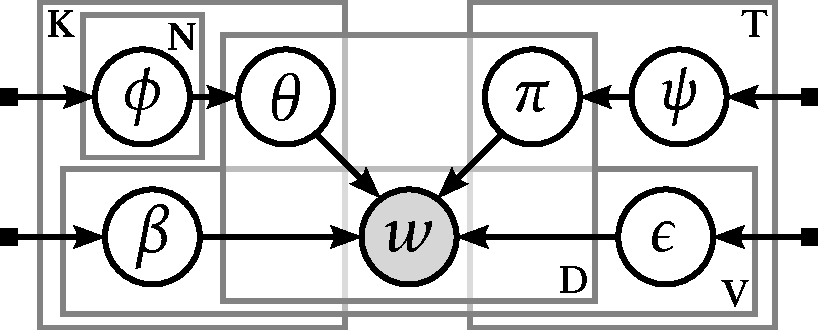
\includegraphics[width=0.5\linewidth]{fig/graphicalmodel.pdf}
\caption{Graphical model for Capsule. Observed term counts depend on
  general topics $\mathbold{\beta}_1, \ldots, \mathbold{\beta}_K$,
  entity topics $\mathbold{\eta}_1, \ldots, \mathbold{\eta}_A$, and
  event topics $\mathbold{\gamma}_1, \ldots, \mathbold{\gamma}_T$, as
  well as message-specific strengths $\mathbold{\theta}_d$, $\zeta_d$,
  and $\mathbold{\epsilon}_d$.  Variables $\mathbold{\phi}_1, \ldots,
  \mathbold{\phi}_A$ and $\xi_1, \ldots, \xi_A$ represent
  entity-specific strengths, while $\psi_1, \ldots, \psi_T$ allow time
  intervals to be more or less ``eventful.'' Black squares denote
  hyperparameters (unlabeled for visual simplicity).}
\label{fig:graphicalmodel}
\end{figure}

\begin{figure}[!ht]
\begin{mdframed}[userdefinedwidth=3.0in,align=center]
\small
\begin{itemize}[leftmargin=*]
\item for $k= 1, \ldots, K$,
	\begin{itemize}[leftmargin=*]
	\item draw general topic\\ $\mathbold{\beta}_k \sim
          \textrm{Dirichlet}_V (\alpha, \ldots, \alpha)$
	\item for each entity $a=1, \ldots, A$,
		\begin{itemize}[leftmargin=*]
		\item draw entity-specific strength \\$\phi_{ak} \sim \textrm{Gamma}\,(s, r)$
		\end{itemize}
                \end{itemize}
\item for each entity $a = 1, \ldots, A$,
	\begin{itemize}[leftmargin=*]
	\item draw entity topic \\$\mathbold{\eta}_a \sim
          \textrm{Dirichlet}_V (\alpha, \ldots, \alpha)$
	\item draw entity-specific strength \\$\xi_{a} \sim \textrm{Gamma}\,(s, r)$
	\end{itemize}
\item for each time interval $t = 1, \ldots, T$,
	\begin{itemize}[leftmargin=*]
	\item draw event topic\\ $\mathbold{\gamma}_t \sim
          \textrm{Dirichlet}_V(\alpha, \ldots, \alpha)$
	\item draw event strength \\$\psi_{t} \sim \textrm{Gamma}\,(s, r)$
	\end{itemize}
\item for each message $d= 1, \ldots, D$, sent during time interval
  $t_d$ by author entity $a_d$,
	\begin{itemize}[leftmargin=*]
	\item for each general topic $k = 1, \ldots, K$,
		\begin{itemize}[leftmargin=*]
			\item draw message-specific strength
                          \\$\theta_{dk} \sim \textrm{Gamma}\,(s,
                          \phi_{a_d k})$
		\end{itemize}
	\item draw message-specific strength \\$\zeta_{d} \sim \textrm{Gamma}\,(s, \xi_{a_d})$
	\item for each time interval $t=1, \ldots, T$,
		\begin{itemize}[leftmargin=*]
			\item draw message-specific strength \\$\epsilon_{dt} \sim \textrm{Gamma}\,(s, \psi_{t})$
		\end{itemize}
	\item for each vocabulary term $v=1, \ldots, V$,
		\begin{itemize}[leftmargin=*]
			\item set $\lambda_{dv} = \sum_{k=1}^K
                          \theta_{dk} \beta_{kv}  + \zeta_d \eta_{a_d
                            v} + {}$\\$ \sum_{t=1}^T f(t_d, t)\, \epsilon_{dt} \gamma_{tv}$
			\item draw term counts \\$n_{d,v} \sim \textrm{Poisson}\left(\lambda_{dv}\right)$
		\end{itemize}
	\end{itemize}
\end{itemize}
\end{mdframed}
\caption{Generative process for Capsule. We use $s$ and $r$ to denote
  top-level (i.e., fixed) shape and rate hyperparameters; they can be
  set to different values for different variables.}
\label{fig:generative-model}
\end{figure}

Given a corpus of messages, learning the posterior distribution of the
latent variables uncovers the three types of topics, the message- and
entity-specific strengths, and the event strengths. In
\cref{sec:detecting}, we explain how an analyst can use the event
strengths as a filter that isolates potentially significant messages.

\subsection{Learning the Posterior Distribution}

In order to use Capsule to to explore a corpus of messages, we must
first learn the posterior distribution of the latent variables---the
general topics, the entity topics, the event topics, the message- and
entity-specific strengths, and the event strengths---conditioned on
the observed term counts. As for many Bayesian models, this posterior
distribution is not tractable to compute; approximating it is
therefore our central statistical and computational problem. We
introduce an approximate inference algorithm for Capsule, based on
variational methods~\cite{Jordan:1999},\footnote{Source code:
  \url{https://github.com/ajbc/capsule}.}, which we outline in
\cref{sec:inference}.\footnote{Appendices are in the supplemental
  material.} This algorithm produces a fitted variational distribution
which be can then be used as a proxy for the true posterior
distribution.

\subsection{Detecting and Characterizing Events}
\label{sec:detecting}

Having approximated the posterior distribution of the latent
variables, we can use the mean of this distribution to explore the
data. Specifically, we can explore ``business-as-usual'' content using
the posterior expected values of the general topics
$\mathbold{\beta}_1, \ldots, \mathbold{\beta}_K$ and the entity topics
$\mathbold{\eta}_1, \ldots, \mathbold{\eta}_A$, and we can detect and
characterize significant events using the posterior expected values of
the event strengths and event topics.

%Once we estimate the posterior distribution of the Capsule parameters, described in the following section, we can use the expectations of the latent parameters to explore the original data.  To detect events, we consider the proportion of the document about event $j$, and take a weighted average of these proportions:
%\begin{equation*}
%m_j = \frac{1}{\sum_{d} f(i_d, j)} \sum_{d}\frac{\varepsilon_{d,j}}{\zeta_d + \sum_{t} \varepsilon_{d,t} + \sum_{k} \E[\theta_{d,k}] },
%\label{eq:eventness}
%\end{equation*}
%where $\varepsilon_{d,t} = f(i_d, t) \E[\epsilon_{d,t}]$.
TODO... This measure of ``eventness'' estimates the fraction of term
occurrences that are related to the event in time interval
$t$. \Cref{fig:cables_events} illustrates real-world events detected
using this measure.

We can characterize an event  $t$ by selecting the highest-probability
vocabulary terms from $\E[\mathbold{\gamma}_t]$. We can also identify
the most strongly-associated messages by computing $f(t_d,
t)\,\E[\epsilon_{dt}]$ for each message $d$ and sorting the messages
accordingly. In \cref{sec:eval}, we explore the cables associated with
significant events in the National Archives' corpus of diplomatic
cables. To make Capsule more accessible for historians, political
scientists, and journalists, we have released an open-source tool for
visualizing its results.\footnote{Source code:
  \url{https://github.com/ajbc/capsule-viz}; demo:
  \url{http://www.princeton.edu/~achaney/capsule/}.} This tool allows
analysts to browse a corpus of messages and the mean of the
corresponding posterior distribution, including general topics, entity
topics, and event topics. \Cref{fig:viz} contains several screenshots of
the tool's browsing interface.

\begin{figure}
\centering
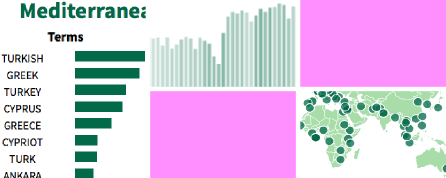
\includegraphics[width=\linewidth]{fig/viz.png}
\caption{Screenshots of the Capsule visualization tool used to explore
  U.S. State Department cables. Top left: events over time (similar to
  \Cref{fig:cables_events}). Top right: entities located on a
  map. Bottom: summary of the week of May 12, 1975, including top
  vocabulary terms, relevant cables, and text from Wikipedia.}
\label{fig:viz}
\end{figure}


%\section{Evaluation}
%\label{sec:eval}
%!TEX root = emnlp2016.tex


% *** results ***
% (1) 1970s cables data; details
%     how we trimmed; how we selected the vocabulary
% (2) we fit the model; 100 topics
%     what we found
% (3) simulations
%     (a) how we simulated data; size, etc.
%     (b) competing methods
%     (c) results

% - divde into pghs
% - made f clear on our model
% - make comparison methods clear (citations)
% - make evaluation metrics clear (citation?)
% - how long does it take to fit the model
% - address simulate then fit
% - details on simuated data; do other methods scale?

% ========================

\PP In this section we first explore the performance of Capsule on a collection of U.S. State Department diplomatics cables, then we ??? on simulated data.

\parhead{Data.}
The National Archive collects communications between the U.S. Sate department and its embassies.  We obtained a collection of these diplomatic messages from the History Lab at Columbia,\footnote{http://history-lab.org} which received them from the Central Foreign Policy Files at the National Archives.  The communications in this data set were sent between 1973 and 1978.

In addition to the text of the cables themselves, each document is supplemented with information about who sent the cable (e.g., the State Department, the U.S. Embassy in Saigon, or an individual by name), who received the cable (often multiple entities), and the date the cable was sent.  We used a vocabulary of size 6,293 and omitted cables with fewer than three terms, resulting in a collection of 2,139,324 messages sent between 27,134 entities.  We selected a weekly duration for the time intervals, as few cables were sent on the weekends.

\parhead{Model settings.}
We fit Capsule with $K=100$ general topics and using an exponential decay $f$,
\begin{equation}
f(i_d, t) = 
\begin{cases}
    0,			& \text{if } t > i_d\\
    \exp\{-(i_d - t) / \tau\},          & \text{otherwise,}
\end{cases}
\end{equation}
with mean lifetime $\tau=3$.  This mean lifetime indicates that most intervals would no longer be relevant after about three weeks.  With these settings on the cables data, fitting the model takes 2.8 hours per iteration;\footnote{Our algorithm is batch--we consider each data point for every iteration.  Modifying the algorithm to stochastically sample the data would reduce the time required to achieve an equivalent model fit.} results are shown on 15 iterations.

\parhead{Results.}
We begin our exploration by detecting events using Capsule.  With Equation~\ref{eq:eventness} as our metric of ``eventness,'' we consider this metric over time, which is shown in Figure~\ref{fig:cables_events}.  Here, peaks correspond to real-worlds events, several of which are labeled.\footnote{Appendix~\ref{sec:additional_results} contains an analogous figure on arXiv data, which shows that Capsule does not capture weekly events on data that does not contain real-world events at that resolution.}

The tallest peak occurs the week of December 1, 1975, just prior to the Indonesian invasion of East Timor, which began December 7, 1975.  As discussed in Section~\ref{sec:model}, we sort documents by their event relevancy parameters $\epsilon$ to find cables that reflect an event.  Table~\ref{tab:timor} shows the top cables for the East Timor invasion.  Capsule accurately identifies this real-world event and recovers relevant cables.

\begin{table*}[tb]
\small
\centering
\begin{tabular}{cccl}
\toprule
$\epsilon$ & date & entity & subject \\
\midrule
0.124   &  1975-12-03  &  State  & President's talking point on Portuguese Timor \\
%0.121   &  1975-12-03  &  State  & President's talking point on Portuguese Timor \\
0.115   &  1975-12-04  &  State  & Timor we are repeating FYI a DAO message \\
0.112   &  1975-12-04  &  State  &  Legal problems relating to Portuguese Timor\\
0.105   &  1975-12-04  &  Secretary Peking & US Support for Timor resolution \\
0.102   &  1975-12-07  &  State  & Invasion of Portuguese Timor \\
\bottomrule
\end{tabular}
\label{tab:timor}
\caption{Top documents for the time interval of week December 1, 1975, just prior to the Indonesian invasion of East Timor, which began December 7, 1975.}
\end{table*}

\begin{table*}[htb]
\small
\centering
\begin{tabular}{cccl}
\toprule
$\epsilon$ & date & entity & subject \\
\midrule
0.090   &  1975-04-24  &  Mansfield, Mike & Assistance in evacuating family from South Vietnam \\
0.089   &  1975-04-24  &  Railsback, Tom & Assistance in evacuating friend from South Vietnam \\
%0.088   &  1975-04-24  &  Mansfield, Mike  & Assistance in evacuating family from South Vietnam \\
%0.086   &  1975-04-24  &  Williams, Harrison &  Assistance in evacuating family from South Vietnam \\
0.086   &  1975-04-24  &  Koch, Edward & Assistance in evacuating family from South Vietnam \\
0.086   &  1975-04-21  &  Schweiker, Richard & Support in evacuating family from Vietnam \\
%$\vdots$ & $\vdots$ & $\vdots$ & $\vdots$ \\
0.081   &  1975-04-25  &  Ketchum, William & Movement of South Vietnamese refugees to Guam \\
0.080   &  1975-04-21  &  Scott, Hugh & Whereabouts of missionaries in Vietnam \\
\bottomrule
\end{tabular}
\label{tab:saigon}
\caption{Top documents for the time interval of week April 21, 1975, just prior to the fall of Saigon on April 30, 1975.}
\end{table*}

The second tallest peak occurs the week of April 21, 1975, just prior to the fall of Saigon on April 30, 1975; Table~\ref{tab:saigon} shows the top cables for this event, which reflect the evacuation efforts that occurred during that week.  Unlike the East Timor event, where the most relevant communication exists at an administrative level, the evacuation of Saigon is best captured by individuals seeking help for family and friends.

Another event peaks occurs the week of July 2, 1973; the top three words under event its description $\pi$ are \emph{bicentennial}, \emph{hijack}, and \emph{mercenary}.  Top cables under event relevancy $\epsilon$ surround the bicentennial celebration of United States (July 4, 1973) and the Air France hijacking incident that began on June 27: Israeli operatives rescued hostages from this incident on July 4th.

Capsule also identifies events with smaller peaks, such as the death of Mao Tse-tung.  One of the top cables for this event is sent by Kissinger to all post with public affairs guidance: %the subject \emph{Death of Mao Tse Tung -- Public Affairs Guidance}:
\begin{shaded*} \tt{1.  Missions should avoid all speculation about the 
possible effects of the death of Chairman Mao on
US-PRC relationships as well as impact on internal
Chinese developments.}

\tt{2.  Official comments should be limited to the statements
of top level administration officials, texts of which
will follow by SEPTEL and wireless file.}
\end{shaded*}
\noindent In the other top cables for this event, embassies generally reported on press reactions and condolence or memorial ceremonies at their various locations.

Capsule helps discovers events which follow a chain of related incidents, though connecting these events is left to the investigator.  For example, Capsule discovers an event the week the Sinai Interim Agreement was signed (September 4, 1975), but it also detects an event in mid-October 1975 about the hiring of observers and technicians for the Sinai peace keeping force.  Associated with this second event is a cable from London to the State department entitled \emph{FCO views on Syrian stance}:
\begin{shaded*} \tt{Since conclusion of Sinai II negotiations, FCO
officials have expressed considerable interest in prospects
for next US effort to promote Syrian negotiations with Israelis. ...}
%Basic FCO position remains one of pervasion admiration for success of 
%Secretary's tactics with Egyptians and Israelis tempered by recognition that
%Syrian negotiating position will be a very tough nut to crack.  
%During recent ...}
\end{shaded*}
\noindent This cable and the sequence of events discovered by Capsule indicate that there is a longer lasting underlying situation.  Capsule cannot capture every aspect of these larger sequences of events, but it can provide insight into key moments so that investigators can explore both short-lived events and long-lasting political situations.

Appendix~\ref{sec:additional_results} contains additional examples of events discovered by Capsule, including results for the Apollo 17 lunar gifts, the return of the crown of St. Stephen to Hungary, and the UN Special Session on Disarmament in 1978.

\begin{table}
\centering
\small
\begin{tabular}{c}
\toprule
top terms \\
\midrule
outlook, review, hire, personnel, invite, prepare \\
arrest, incident, security, family, guard, death, jail \\
locate, home, son, death, please, contact, father \\
request, refugee, response, service, sale, asylum \\
market, report, commercial, food, import, commerce \\
fear, leadership, back, arm, role, threaten \\
hotel, travel, reservation, visit, arrange, schedule \\
\bottomrule
\end{tabular}
\label{tab:topics}
\caption{Top vocabulary terms for a selection of topics, one per row, according to topic distributions $\beta_k$.}
\end{table}

\begin{table}
\centering
\small
\begin{tabular}{cc}
\toprule
entity & top terms \\
\midrule
State & request, follow, embassy, meet, make \\
Bangkok & bangkok, thailand, thai, refugee, follow \\
Jerusalem & jerusalem, israeli, bank, report, say \\
Stockholm & swedish, sweden, trade, meet, embassy \\
%Casablanca & casablanca, morocco, moroccan, request, please, note \\
Kampala & ugandan, nairobi, african, imperialist \\
Ndjamean & chadian, chad, lagos, drought, austerity \\
\bottomrule
\end{tabular}
\label{tab:entities}
\caption{Top vocabulary terms for a selection of entities according to entity-exclusive topics $\beta^{(n)}_0$.}
\end{table}

In addition to events, Capsule can be used to explore the general themes in the corpus and the concerns of specific entities.  Examples of general topics of conversation are shown in Table~\ref{tab:topics} and entity-exclusive topics are shown in Table~\ref{tab:entities}; these show us how entity topics absorb location-specific words, preventing these terms from overwhelming the general topics.  Appendix~\ref{sec:additional_results} contains more examples of general and entity-specific topics.

These exploratory results show that our model is successfully capturing when multiple entities are discussing the same subjects and that our model can be used to explore the underlying data by providing a structured scaffold from which to view the data.



\parhead{Simulations.}
\PP how did we simulate data; note on why this is okay

\PP evaluation metrics; w/ citations

\PP comparison methods; w/ citations

\PP eventness results

\PP document recovery results

\PP note on sensitivity to duration/shape and more simulations in Appendix~\ref{sec:additional_results}



\begin{figure}[h]
\centering
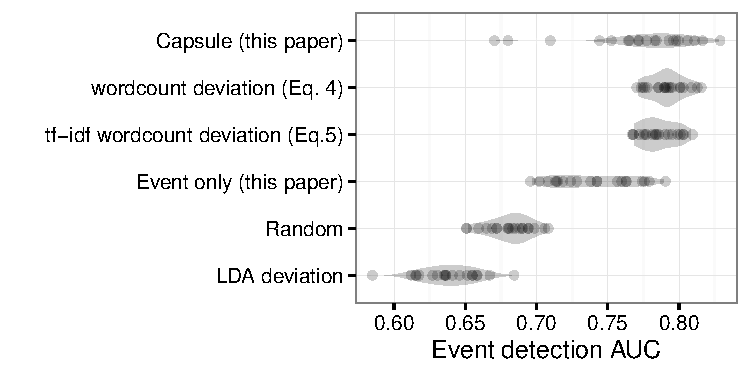
\includegraphics[width=\linewidth]{fig/sim_eventdetect.pdf}
\caption{Event detection performance on twenty simulated datasets.  Capsule is able to detect events as well as comparison methods, but its performance has higher variance.}
\label{fig:sim_eventdetect}
\end{figure}

Finally, we simulated data according to our generative process in order to compare our method to baseline and existing approaches.  
To evaluate event detection, we created a ranked list of all time intervals and computed the overlap between a model and the simulated ground at every threshold; this generates an curve under which we cam compute the area and normalized based on ideal performance---we refer to this metric as event detection AUC.  
The most successful of the comparison methods for event detection was average absolute error in wordcount, both unweighted and weighted by tf-idf.  Figure~\ref{fig:sim_eventdetect} shows that Capsule can outperform these approaches for event detection, but that it has higher variance in performance.  The other comparison method in Figure~\ref{fig:sim_eventdetect} is based on LDA; we fit a multinomial Gaussian to the topic representation of all documents and then computed the average probability of seeing the topic distributions of documents in the time interval.  Time intervals with the lowest probability were marked as most likely to have events.  All other baselines performed close to random for event detection.
\begin{figure}[h]
\centering
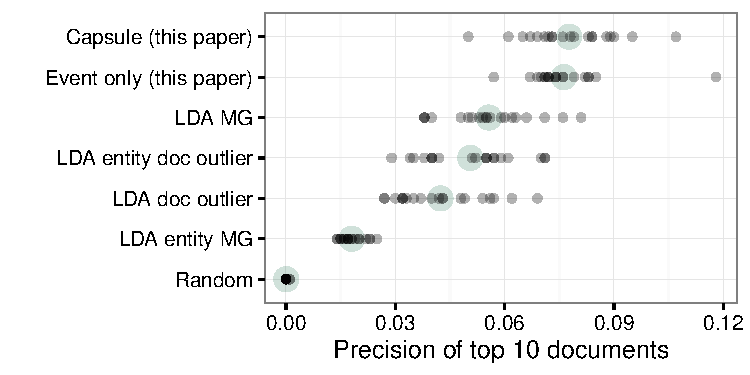
\includegraphics[width=\linewidth]{fig/precision10.pdf}
\caption{Precision of recovering the top ten most relevant documents, averaged over all time intervals.  Capsule performs best, averaged over twenty simulations.}
\label{fig:sim_precision}
\end{figure}

This method of fitting a multinomial Gaussian to LDA representations of documents also performed well for recovering relevant documents.  This approach can be altered to fit a per-entity multinomial Gaussian, but this performs worse.  Simply finding documents based on absolute deviation from the mean works well in LDA topic space (relative to overall mean or entity mean), but not over the full vocabulary.  Word count deviations, which performed well for event detection, performed worse than random for document recovery.  Both Capsule and its event-only partial model outperform all comparison methods in terms of document recovery.  Figure~\ref{fig:sim_precision} shows precision of recovering the top ten documents.

We assessed the sensitivity of our model to three different decay functions $f$: exponential, linear, and step functions.  We simulated data for each function and then fit Capsule using every permutation of $f$ and multiple settings for event decay duration.  In all cases, we found that the model is not sensitive to decay shape or duration.

% \begin{figure*}
% \centering
% 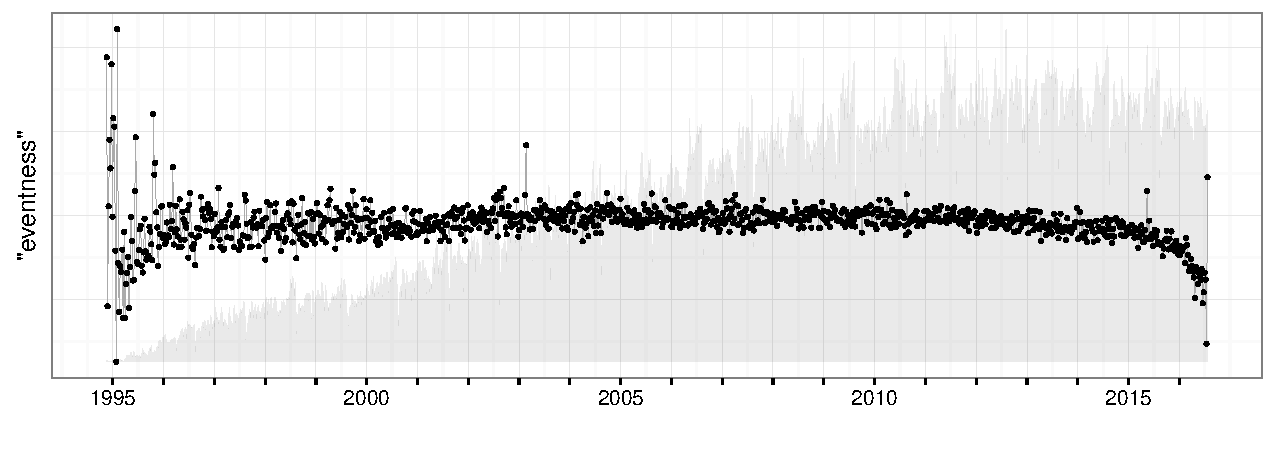
\includegraphics[width=\linewidth]{fig/arxiv_events.pdf}
% \caption{TODO}
% \label{fig:arxiv_events}
% \end{figure*}






% In this section we study the performance of Capsule. Using simulated data, we compare Capsule to deterministic methods of event detection and show that Capsule outperforms them at identifying when events occur.  
% %We also examine how sensitive Capsule is to the attributes of a dataset and model parameters.
% We conclude by exploring three real-world datasets with Capsule.

% \subsection{Performance}

% We generated ten simulated datasets using our generative process.  Each dataset spans 100 days and contains content associated with ten entities.  Approximately ten events also exist in each dataset, randomly distributed in time and with a three day decay of relevancy.

% To evaluate performance, we rank each day by its probability of having an event occur, and plot the number of true events discovered against the number of false positive events, as shown in Figure~\ref{fig:sim_auc}; the area under the curve (AUC) can be computed for a single evaluation metric.  Note that this approach is only valid when true events are known, and thus we only apply it to simulated data.

% We compare Capsule to two baseline approaches: one considers the greatest document outlier on a given day--days with the furthest outliers are the most likely to have events.  The other approach is similar: days are represented by an average of all documents associated with that day, and one considers how these averages deviate from the global average--the further away, the more likely an event.

% Figure~\ref{fig:sim_auc} shows that Capsule outperforms both of these approaches.  It should be noted that inference on Capsule will produce different results, depending on the random seed; the results shown are the best of three random seeds.

% \begin{figure}[ht]
% \centering
% 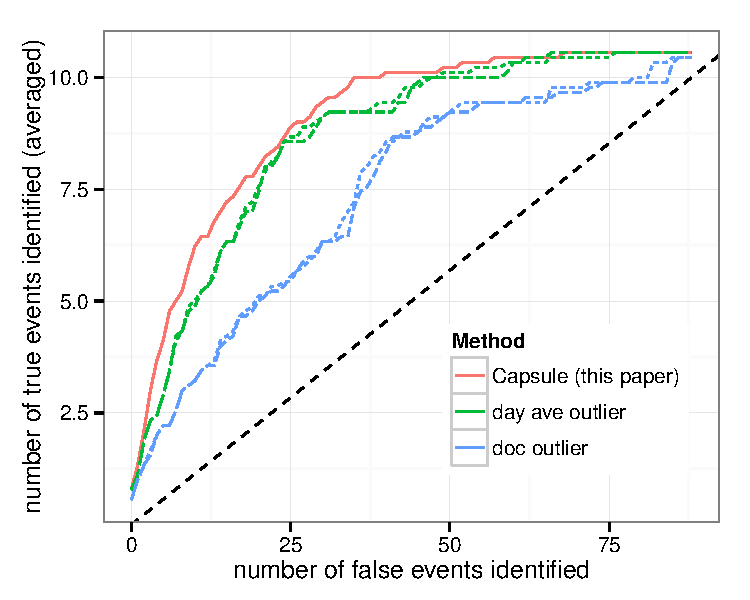
\includegraphics[width=\linewidth]{fig/sim_auc.pdf}
% \caption{Average performance on ten simulated datasets; lines closer to the upper-left are better.  Baselines consider outliers based on full corpus averages (dashed) and averages of all entity documents (dotted).  Capsule performance is best of three random seeds.}
% \label{fig:sim_auc}
% \end{figure}


% %\PP fig / discussion of varrying entity dists in simualted data

% %\PP performance vs parameters (event occurrence hyperparameter (which impacts initialization), event duration)

% \subsection{Exploration}

% \parhead{Cables}
% \PP where did we get it / size / preprocessing

% \PP plot of events timeline with select real-world match evetns pointed out (verified by history lab)

% \PP example interesting entities + figure

% \PP explore pairwise entities? (quick with and single figure shared with enron); compare sender vs reiever for same pair  (or does direction matter?? tyr both ways) look at sender in norma model vs sender in a few pairs under this construction 

% \parhead{arXiv}
% \PP where did we get it / size / preprocessing

% \PP plot of events timeline with select real-world match evetns pointed out (verified by history lab)

% \PP example interesting entities + figure

% \parhead{enron}
% \PP where did we get it / size / preprocessing

% \PP plot of events timeline with select real-world match evetns pointed out (verified by history lab)

% \PP example interesting entities + figure

% \PP explore pairwise entities?



% % \parhead{Cables}
% % We obtained around two million of these cables sent between 1973 and 1977 via the History Lab at Columbia,\footnote{http://history-lab.org} which received them from the Central Foreign Policy Files at the National Archives.  In addition to the text of the cables themselves, each document is supplemented with information about who sent the cable (e.g., the State Department, the U.S. Embassy in Saigon, or an individual by name), who received the cable (often multiple entities), and the date the cable was sent.
% % Excerpts from three example cables are shown in Figure~\ref{fig:cables_example}.

% % % \begin{figure}[ht]
% % % \centering
% % % 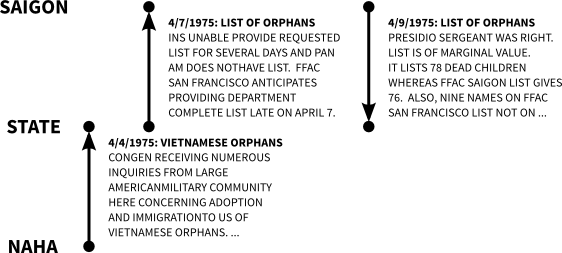
\includegraphics[width=\textwidth]{../fig/cables_orphan_example.png}
% % % \caption{Example excerpts of cables sent in April 1975 concerning orphans from the Vietnam War.}
% % % \label{fig:cables_example}
% % % \end{figure}

% % \parhead{arXiv}

% % \parhead{Enron}


% % \PP insert table and refetence for both (number of days, entities, total messages, or something); maybe a plot showing attributes of the data...somehow inform them that the state department is a bias for the cables data

% % \PP footnote on handling multiple recipients of message...

% % \subsection{Metrics and competing methods}

% % \PP how we evaluate based on real events

% % \PP how we evaluate based on perplexity (prediction of words)

% % \PP competing methods for perplexity: LDA, average user words?, dynamic topic model, network topic models

% % \subsection{Performance and exploration}

% % \PP sumry of comparison to gold-standard events for cables

% % \PP table of predictive likelihood results and summary pgh; and/or cite tea leaves paper

% % \parhead{Exploration}

% % \PP charachetrize events manually (based on cables) vs event detection characterization

% % \PP show descriptions for cables entities and select events; same for arxiv/enron

% % \PP any other exploration you can think of!


% % Results: ROC curve (x=false postive rate, y=true postive rate)

\section{Conclusion}
\label{sec:discussion}
We have presented Capsule, a Bayesian model that identifies when events occur, characterizes these events, and discovers the typical concerns of author entities.  We have shown that Capsule outperforms deterministic baseline methods and explored its results on a real-world datasets.
We anticipate that Capsule %and its visualization
can be used by historians, political scientist, and others who wish to explore and investigate events in large text corpora.  
%Future work includes expanding the model to incorporate messages recipients and allowing events to impact only a subset of entities.

%TODO:
% go through and check citation styles [ ~\cite{Gusfield:97} and Gusfield~\shortcite{Gusfield:97} ]

% \small
\section*{Acknowledgments}
This work was supported by NSF SBE-0965436, IIS-1247664, and
IIS-1320219; ONR N00014-11-1-0651; DARPA FA8750-14-2-0009 and
N66001-15-C-4032; Adobe; the Alfred P. Sloan Foundation; and 
the Columbia Global Policy Initiative.

% Do not number the acknowledgment section. %TODO

\bibliography{library.bib}
\bibliographystyle{emnlp2016}

\end{document}
